% Some LaTeX commands I define for my own nomenclature.
% If you have to, it's better to change nomenclature once here than in a 
% million places throughout your thesis!



%======================================================================
\chapter{Methodology }
%======================================================================

\section{Methodology for achieving Objective - 1 }

\textbf{Objective 1: To understand foreign visitors' attitudes toward Safety Tips.}

 For research objective 1, the nationality data in item 1 and item 6 were used, containing three tasks. While considering that the main users of Safety Tips are foreign visitors, only the sample of foreign respondents was selected for this part of the analysis, and the sample of Japanese respondents was excluded in this part. So the total number of samples was 1500.

The first task is to summarize the questionnaire's results from Q15 to Q17. The findings will show the popularity, experience, and attitude of Safety Tips in each country, as well as the differences among respondents from 5 countries.

The second question was based on the answers to Q15 and Q16, and all respondents were divided into five groups. Q15 was "do you know Safety tips or not?", and Q16 was "Did you use safety tips before or not?". The answers to Q15 had three options: Know exactly, Heard safety tips before, and Do not know. If the respondent answered "Know exactly" or "Heard Safety tips before", the respondent will continue to answer Q16, if the respondent answers "Do not know", the respondent will directly skip to Q17. The answers to Q16 are "used Safety tips before." and "never used it before". Therefore, the respondents were divided into the following five groups: "Know exactly and used Safety tips before", "Know exactly but never used Safety tips before.", "Heard Safety tips before and used it before", "Heard Safety tips before but never used it before", and "Do not know and never used before". The sample sizes for each group are shown in Figure~\ref{fig6}, which are "Know exactly and used Safety tips before": 357; "Know exactly but never used Safety tips before": 90; "Heard Safety tips before and used it before": 134; "Heard Safety tips before but never used it before": 465 people; "Do not know and never used before": 454 people. The results will show whether the two factors of respondents' past awareness and whether they used it before had an impact on their attitudes toward Safety Tips.

\begin{figure*}[h]
  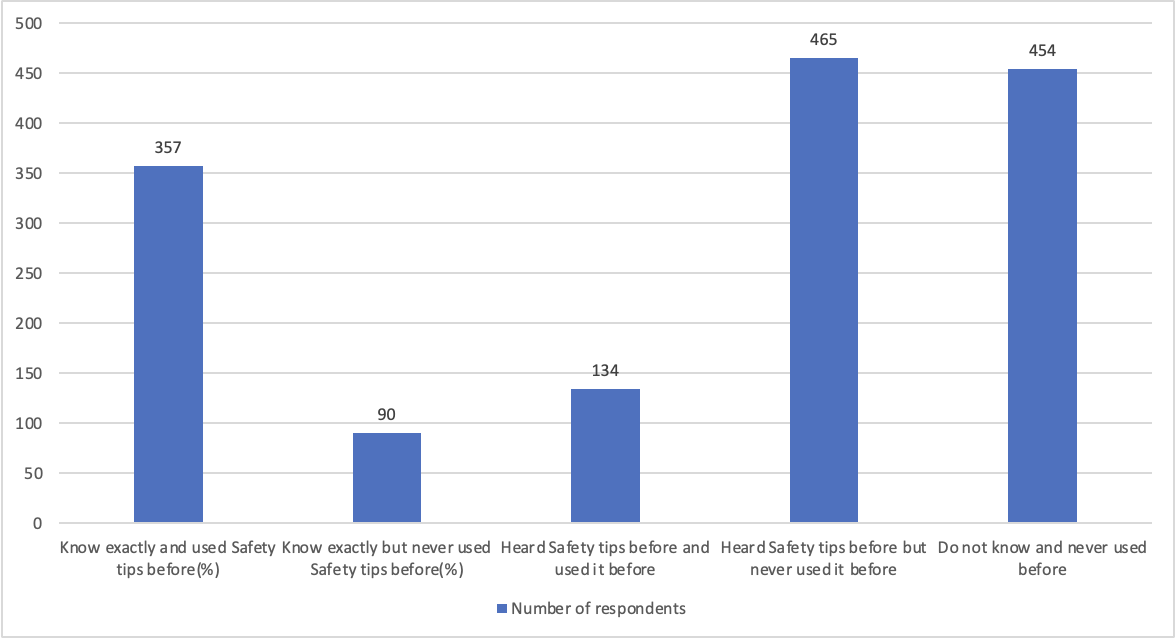
\includegraphics[width=\linewidth]{Figure/Figure6.jpg}
  \centering
  \caption{Number of respondents in each group. }
  \label{fig6}
\end{figure*}

The third task is an independent sample t-test analysis. The responses of Q15 and Q16 were used to test whether the responses of the respondents to the four questions of Q17 were significantly different because of the difference between Q15 and Q16. The independent sample t-test analysis of Q15 versus Q17\_1, Q17\_2, Q17\_3, and Q17\_4 examined whether there were significant differences in the attitudes toward Safety Tips between respondents who were previously aware of Safety Tips and those who were previously unaware of Safety Tips. Independent sample t-tests for Q16 and Q17\_1, Q17\_2, Q17\_3, and Q17\_4 were conducted to examine whether there was a significant difference in attitudes toward Safety Tips between respondents who had previously used Safety Tips and those who had not used Safety Tips.


\section{Methodology for achieving Objective - 2 }
\textbf{Objective 2: To explore how respondents' attitudes toward Safety Tips are influenced by their characteristics. }

For research purpose 2, the data of Item 1, Item 2-4, and Item 6 were used. This part will continue to look into the impact of respondents' personality characteristics on their attitude toward Safety Tips. As a consequence, the study still uses a sample size of 1500 foreign visitors.

Structural Equation Modeling will be used to analyze this part. Structural Equation Modeling is a statistical method based on Regression Models for Latent Variables. Structural Equation Modeling can consider and deal with multiple dependent variables at the same time and allow for measurement error in both independent and dependent variables. Also, Structural Equation Modeling can estimate both factor structure and factor relationships, which could be more useful for this research. Therefore, this study will use Structural Equation Modeling to explore whether factors such as respondents' personal characteristics, disaster consciousness, disaster experience, and disaster training experience will have an impact on respondents' attitudes toward Safety Tips or not. Like \#Table 5 shows, there are four Latent variables, which are Disaster Prevention Consciousness, Disaster Knowledge, and Attitude toward Safety Tips. The latent variable "Disaster Prevention" has 5 manifest variables, which are Disastrous Imagination (Q1), Sense of crisis (Q2), Other-directed type (Q3), Anxiety (Q4), Apathy about disasters (Q5). The latent variable "Disaster knowledge" has 2 manifest variables, which are Knowledge about earthquakes (Q9) and Knowledge of how to respond to a disaster (Q10). The latent variable "Training experiences" has 2 manifest variables, which are the Total score of earthquake/tsunami/typhoon/fire training experiences. (Q6) and Number of times participating in earthquake/tsunami/typhoon/fire disaster training (Q7). The latent variable "Attitude on Safety Tips" has 2 manifest variables, which are Trust level (Q17\_1), Priority of use (Q17\_2), Usefulness (Q17\_3), and Possibility of future use (Q17\_4). There are another 6 manifest variables, which are Age (FQ3), Gender (FQ2), Number of visits to Japan within 1 year (FQ5), Number of visits to any country in the world within 1 year (FQ4), Japanese level (FQ7), and Number of experienced earthquakes (Q8).

\subsection{Hypothesis for SEM}

In order to construct Structural Equation Modeling for this research, it is necessary to make hypothesizes based on previous research.  

\begin{itemize}
\item Individual characteristics (risk belief, connectedness, knowledge, and past experience with hurricanes), travel-related variables, and the socio-demographic characteristics of tourists influence their decision regarding whether or not to evacuate in the event of a hurricane.~\cite{Cahyanto2014AnEE}
\item The tourists' evacuations were also influenced by tourists' hurricane knowledge and past experience.~\cite{Cahyanto2016StatedPO}
\end{itemize}

Base on these two studies, we can construct a relationship that knowledge, travel-related variables, and socio-demographic characteristics could relate to Evacuation Behaviors, shown in Figure~\ref{fig7}. 

\begin{figure*}[h]
  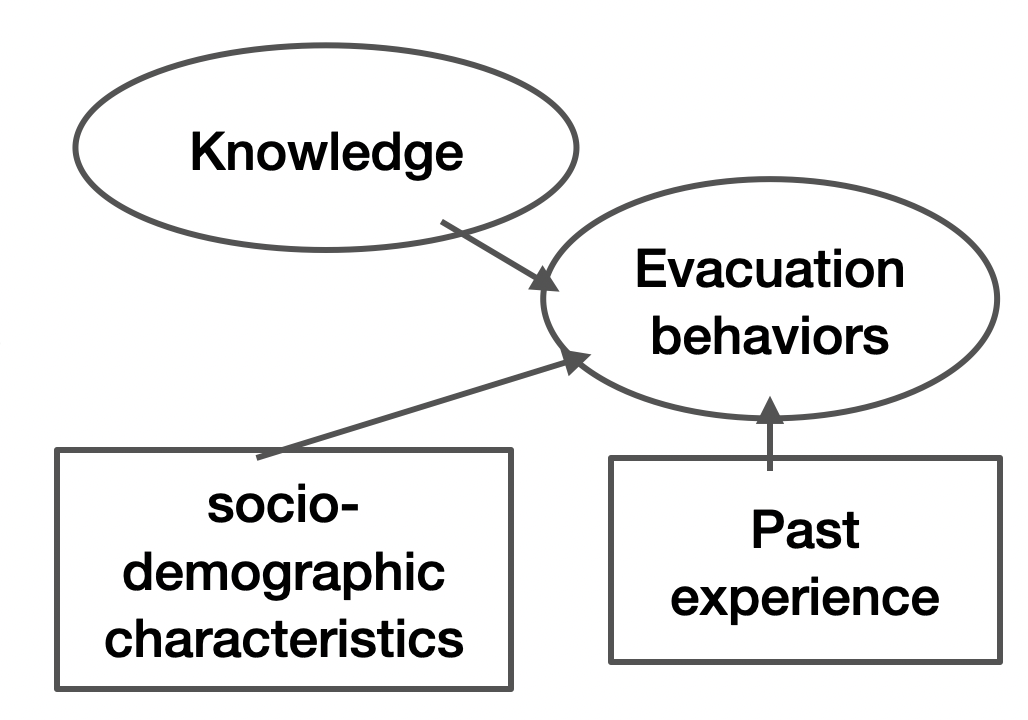
\includegraphics[width=0.5\linewidth]{Figure/Figure7.png}
  \centering
  \caption{Hypothesis base on previous research - 1 }
  \label{fig7}
\end{figure*}

\begin{itemize}
\item Evacuation is significantly related to Socio-demographic factors, such as age, gender, etc, Socioeconomic factors, like educational attainment or household characteristics, etc, Personal characteristics, like hazard experience, knowledge, abilities/impairments, etc. Also, evacuees tend to make use of their familiarity with the surroundings based on their knowledge.~\cite{Wang2021IncorporatingHF}
\end{itemize}

Base on this study, we can construct a relationship that age, gender, hazard experience,  educational attainment, knowledge, abilities could relate to Evacuation Behaviors, shown in Figure~\ref{fig8}. 

\begin{figure*}[h]
  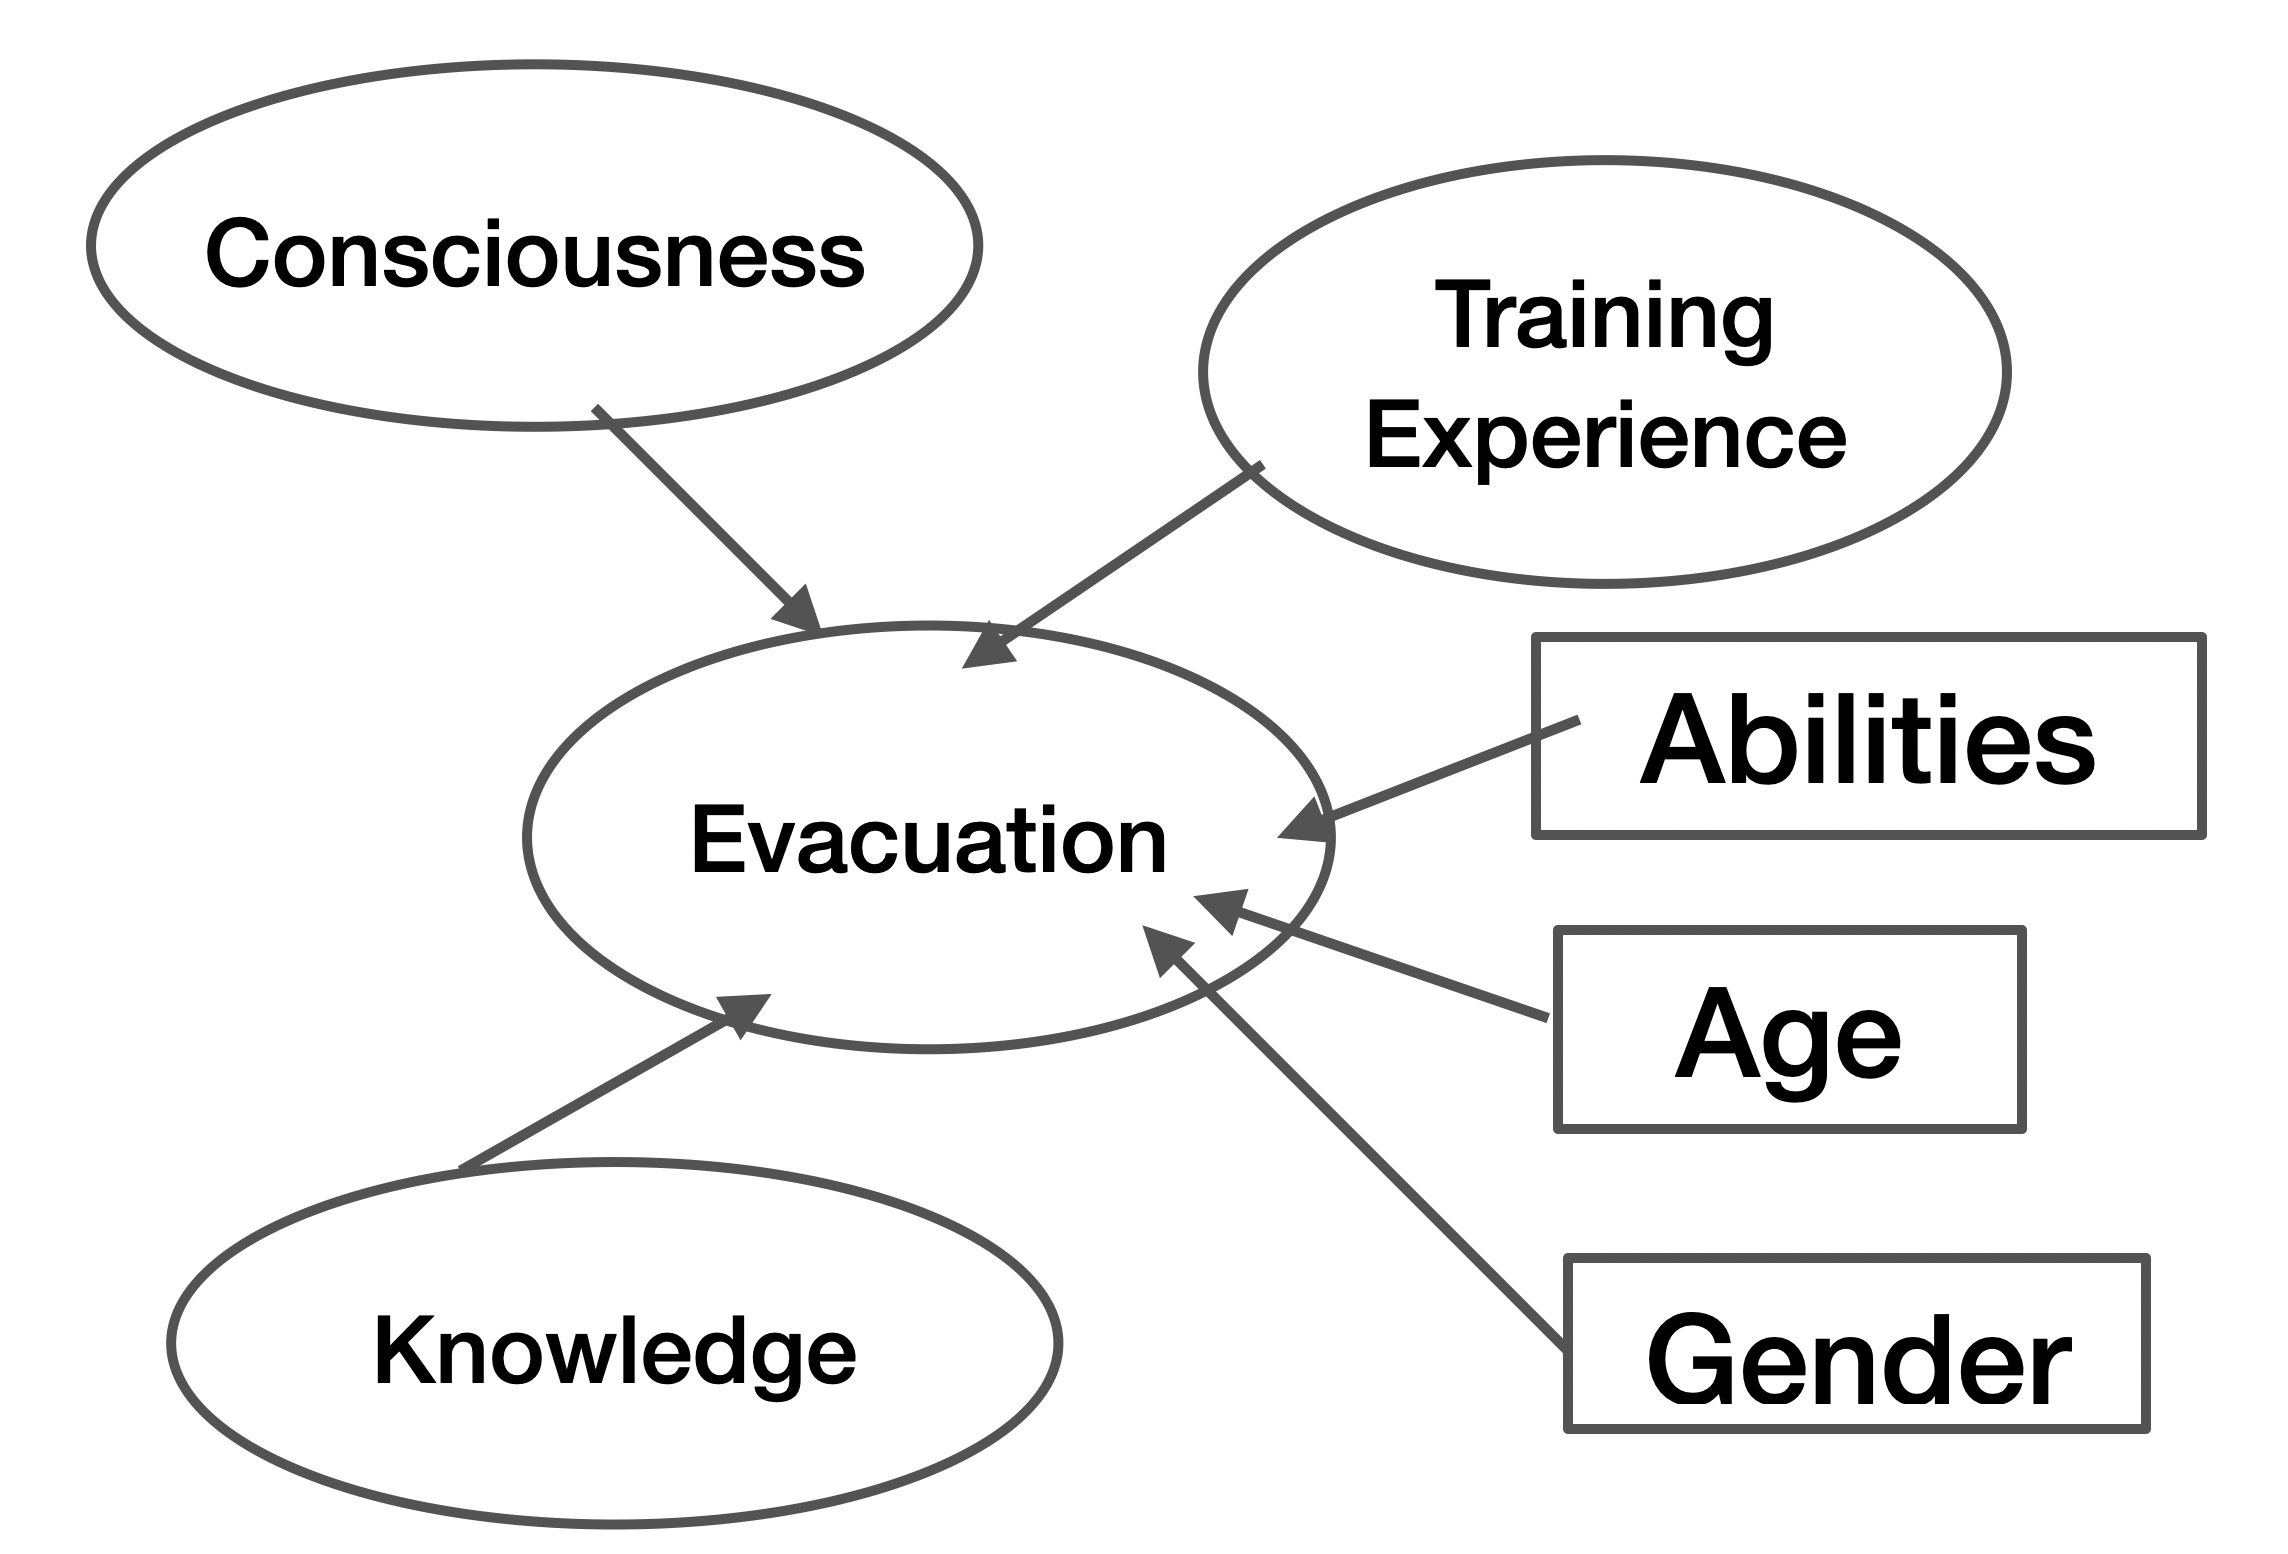
\includegraphics[width=0.5\linewidth]{Figure/Figure8.png}
  \centering
  \caption{Hypothesis base on previous research - 2 }
  \label{fig8}
\end{figure*}

By combining these hypothesizes, we finally construct an SEM model, shown in Figure~\ref{fig9}. 

\begin{figure*}[h]
  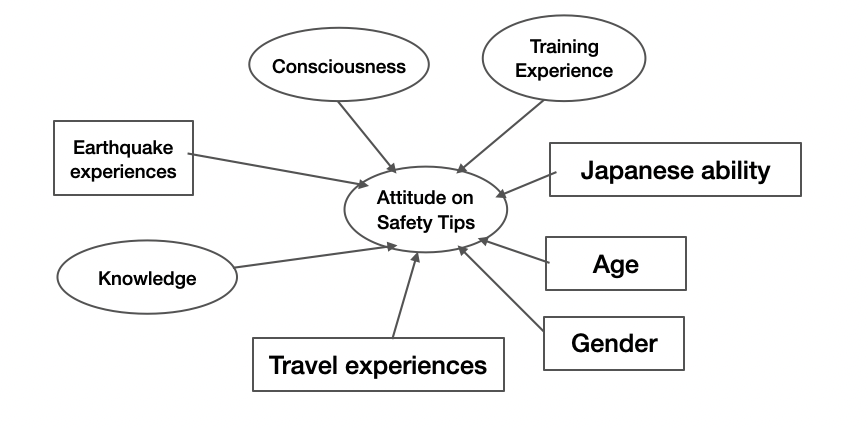
\includegraphics[width=\linewidth]{Figure/Figure9.png}
  \centering
  \caption{Final Hypothesis used for SEM }
  \label{fig9}
\end{figure*}

\subsection{Data Processing}
\begin{itemize}
\item Item 1 (FQ2-FQ5,FQ7)
\end{itemize}

FQ2: $(Male) = 1$; $(Female) = 2$;

FQ3: $(Age Under 15) = 1$; $(Age 16-19) = 2$; $(Age 20-29) = 3$; $(Age 30-39) = 4$; $(Age 40-49) = 5$; $(Age 50-59) = 6$; $(Age 60-69) = 7$; $(Age Over 70) = 8$;

FQ4\&FQ5: number means the time of visit country/Japan;

FQ7: $(Cannot understand) = 1$; $(Basic) = 2$; $(Intermediate) = 3$; $(Up Level) = 4$; 

\begin{itemize}
\item Item 2 (Q1-Q5)
\end{itemize}

Since each of Q1-Q5 has four sub-problems. Here will use the mean values of the four sub-problems as the final data. For example, Q1 = $mean$ (Q1\_1, Q1\_2, Q1\_3, Q1\_4), Q2-Q5 are processed in the same way.

\begin{itemize}
\item Item 3 (Q6-Q8)
\end{itemize}

Q6 is about past disaster training participation experience. There are four types of disasters: Q6\_1 earthquake, Q6\_2 tsunami, Q6\_3 typhoon, and Q6\_4 fire. Each of them has 12 different types of training experience, shown as Q6\_1/2/3/4\_1 to Q6\_1/2/3/4\_12. Respondents answered with 'Yes' or 'No' in these questions. If none of them were experienced before, 'Yes' was selected in Q6\_1/2/3/4\_13 to indicate that the respondent did not have any of the 12 experiences mentioned above. 

Therefore, 

Q6\_1 = $sum$ (Q6\_1\_1 + Q6\_1\_2 +... + Q6\_1\_12);

Q6\_2 = $sum$ (Q6\_2\_1 + Q6\_2\_2 +... + Q6\_2\_12);

Q6\_3 = $sum$ (Q6\_3\_1 + Q6\_3\_2 +... + Q6\_3\_12);

Q6\_4 = $sum$ (Q6\_4\_1 + Q6\_4\_2 +... + Q6\_4\_12).

Q7 is times of past disaster training experiences. There are also four types of disasters: Q7\_1 earthquake, Q7\_2 tsunami, Q7\_3 typhoon, and Q7\_4 fire.
 
(one time) = 1; (2-3 times) = 2; (4-6 times) = 3; (Over 7 times) =4;

\begin{itemize}
\item Item 4 (Q9-Q10)
\end{itemize}

Q9 has six sub-problems, Q10 has nine sub-problems. Here will use the mean values of the sub-problems as the final data. 

Therefore, 

Q9 = $mean$ (Q9\_1, Q9\_2, ... , Q9\_6);

Q10 = $mean$ (Q10\_1, Q10\_2, ... , Q10\_9).

\begin{itemize}
\item Item 6 (Q15-Q17)
\end{itemize}

Q15: (Don't know) = 1; (Only heard name before) = 2; (Know exactly) = 3;

Q16: (Never used before) = 0; (Used before) = 1;
 
Q17\_1, Q17\_2, Q17\_3, Q17\_4: use orginal data.


\section{Methodology for achieving Objective - 3}

\textbf{Objective 3: To explore patterns of information seeking and evacuation behaviors.}

For research objective 3, this study wanted to explore respondents' information-seeking behaviors and evacuation behaviors through their selections of behaviors. In order to understand which of the behaviors are preferred and which are selected more frequently, we chose to measure both the selected rate and the selected score. The calculation of the selected rate and the selected score will both do three times, for 300 Japanese samples, 1500 foreign visitors samples, and 1800 of all respondents' samples.

\subsection{Selected Rate}
Because the selected rate wants to explore which behaviors are used more, this part does not take the order factor into account. No matter the behavior is selected in which order, it will count as 1 point. The selected rate is equal to the Sum selected point divided by the sample number, shown in Figure~\ref{fig10}.

\begin{figure*}[h]
  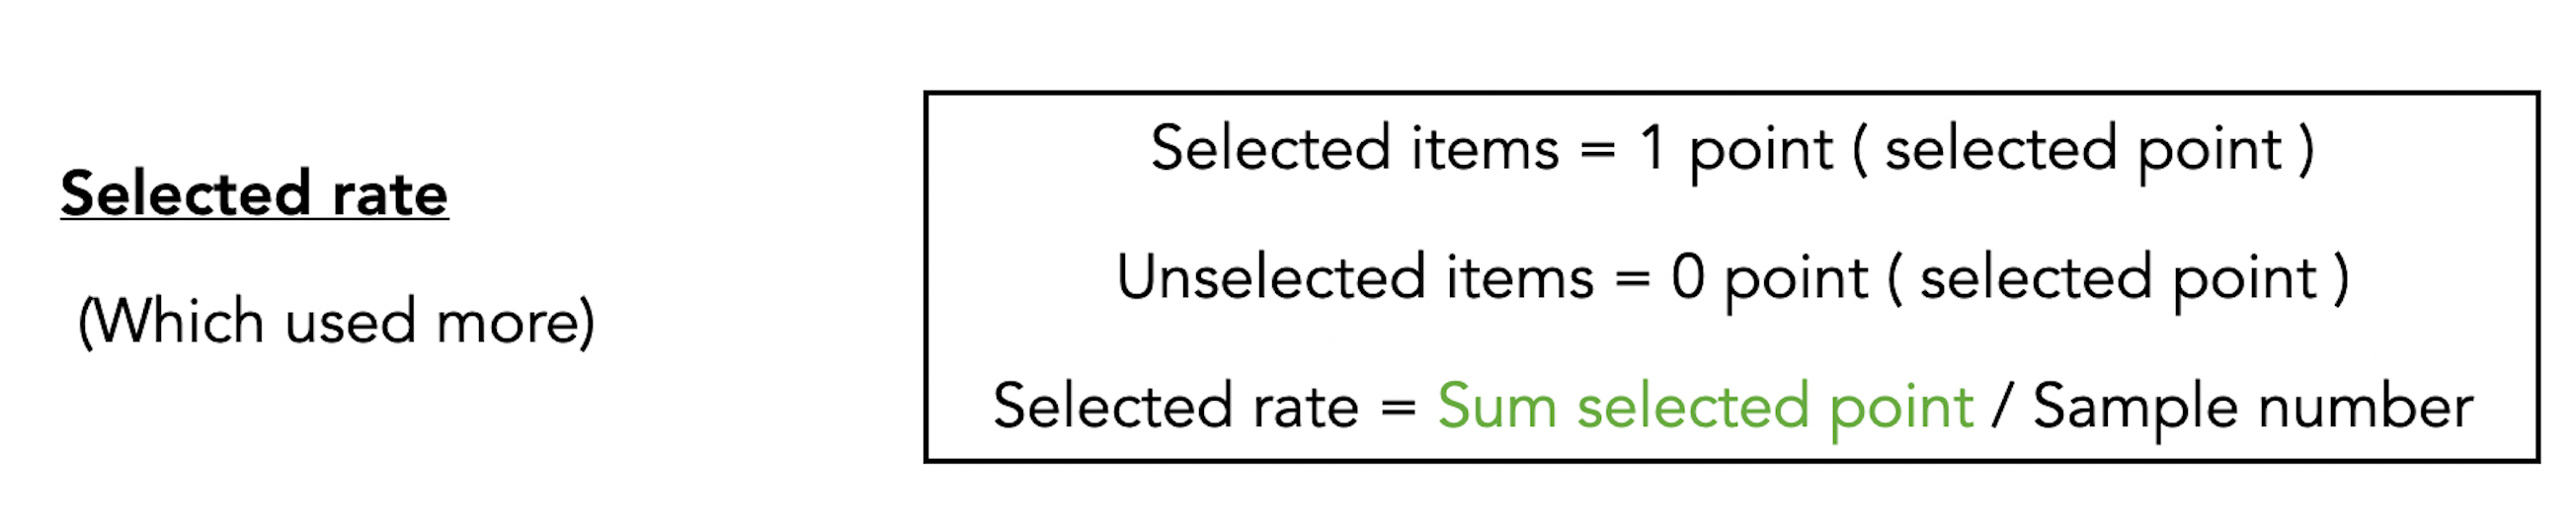
\includegraphics[width=\linewidth]{Figure/Figure10.png}
  \centering
  \caption{Selected rate }
  \label{fig10}
\end{figure*}

\subsection{Selected Score}

Since the Selected score wants to explore which behaviors are used first, this part needs to take the order factor into account. The higher the preference is, the higher the score will be. So the first selected action is scored as 5, the second is scored as 4, the third is scored as 3, the fourth is scored as 2, and the last selected action is scored as 1. The Selected score is equal to the total score divided by the Sum selected point, shown in Figure~\ref{fig11}.

\begin{figure*}[h]
  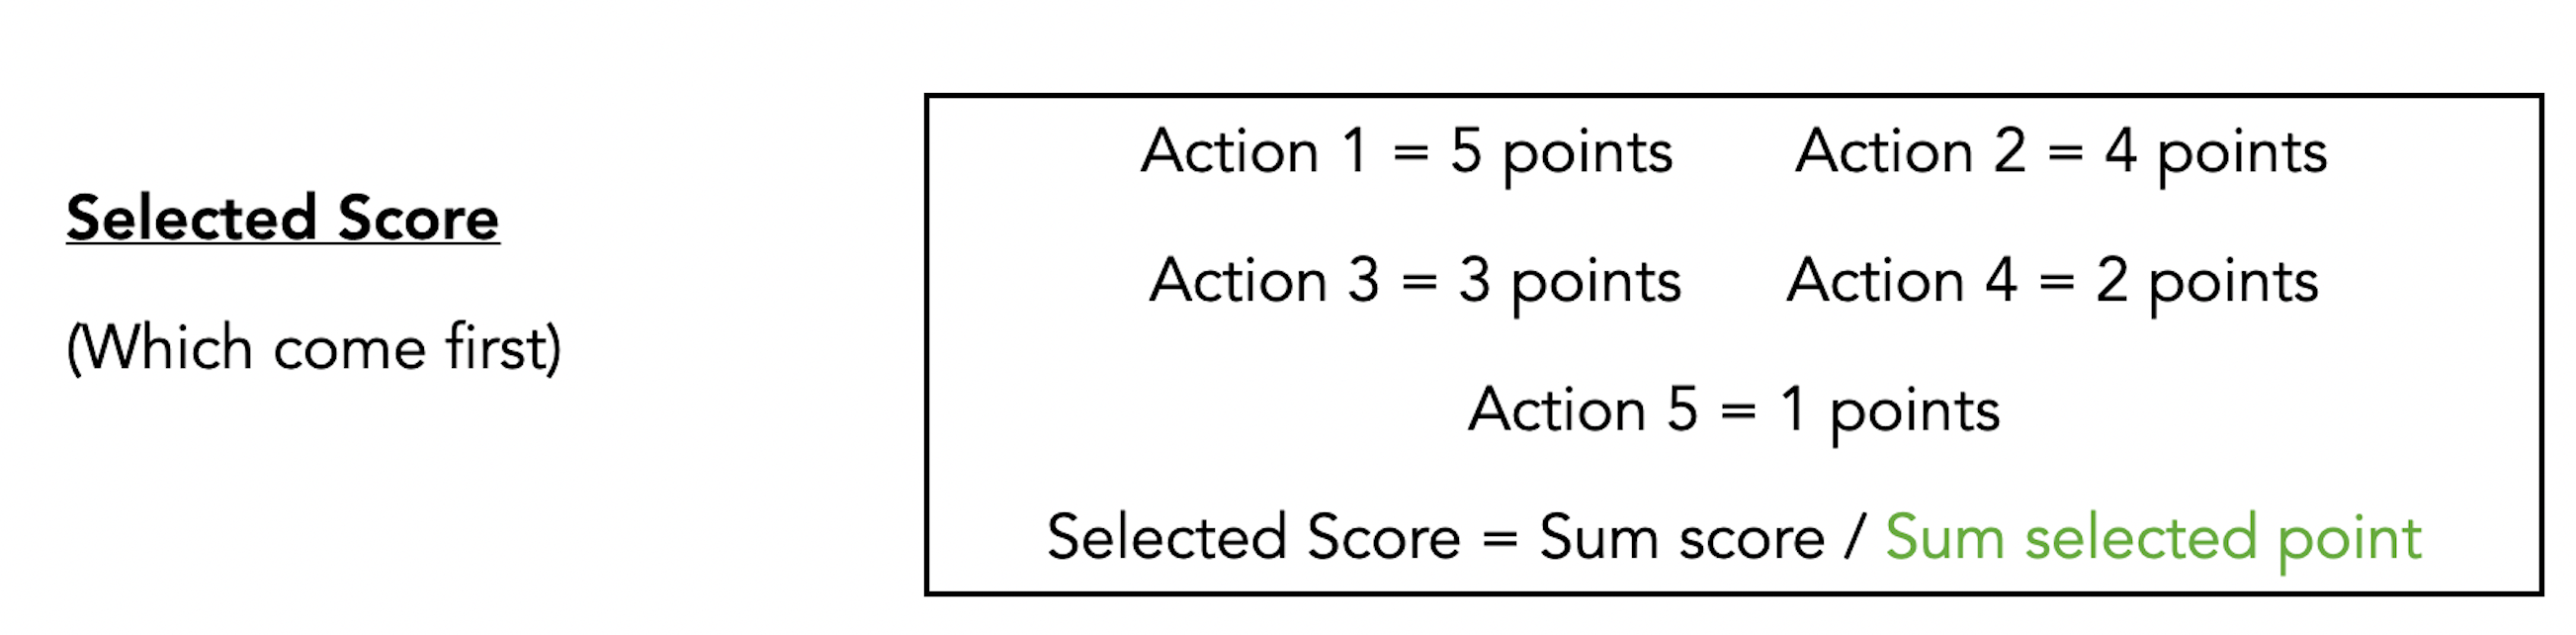
\includegraphics[width=\linewidth]{Figure/Figure11.png}
  \centering
  \caption{Selected score}
  \label{fig11}
\end{figure*}

\subsection{Behavior Pattern}

In the analysis of the selected score and selected rate of study objective 3, we will find that all the results will be relatively scattered. This is because, in this study, the number of available selections is relatively large, which makes the results more scattered. However, from the results, we can see that there could be similarities in the behavior patterns of people. Here the word "pattern" means behavior patterns, not specific behavior. For example, the behavior of  "collecting information" is the same, the difference is how to collect information, from official websites, from disaster prevention software, from disaster prevention websites, from SNS, etc. So how to divide detailed behaviors into patterns? From the available selection, we can find that the behavior is mainly divided into two kinds, which are information-seeking behavior and evacuation behavior. First, regarding information-seeking behavior, we can find that there are two main patterns, one is "No-face-to-face information seeking" and the other is "Face-to-face information seeking". And for the evacuation behavior, we can also find two main patterns, one is " Self-evacuation behaviors " and the other is " Following evacuation guidance behavior ". Then, we divided all the selections into the patterns they belong to, which can be found in Figure~\ref{fig12}.

\begin{figure*}[h]
  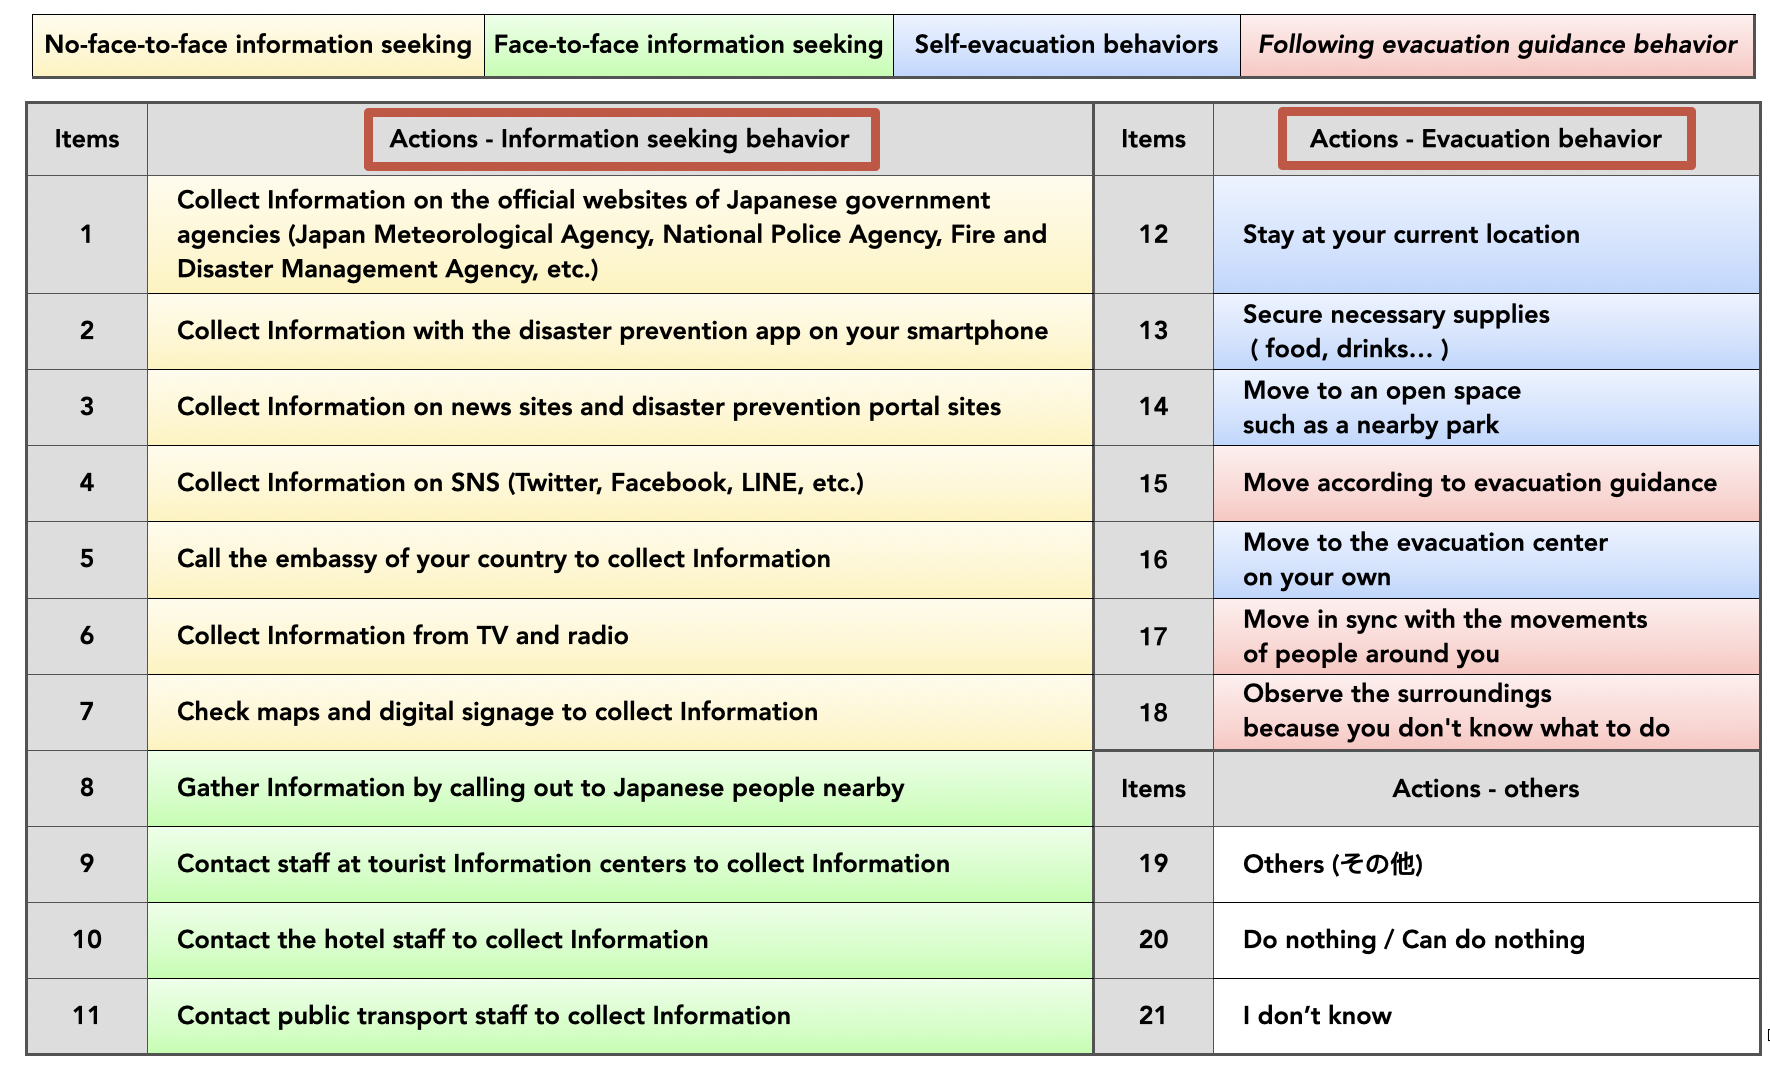
\includegraphics[width=\linewidth]{Figure/Figure12.png}
  \centering
  \caption{behavior patterns}
  \label{fig12}
\end{figure*}

After attributing all the actions to the 4 patterns, we went through the flow of the respondents' actions with the help of the Sankey Program. The Sankey Program is a flow chart that shows the flow from each set of values to another set of values. The thickness of the lines expresses the number of values present in the group. In the Sankey Program, the number indicates the No. of action, so 1-5 means the first action to the fifth action. Capital letters indicate behavior patterns." No-face-to-face information seeking" is A; "Face-to-face information seeking" is B; "Self-evacuation behaviors" is C; "Following evacuation guidance behavior" is D. Thus, the behavior from the first to the fifth cohort can be clearly represented in the results of the Sankey Program. As an example, A1 indicates that the 1st response action during the disaster is behavior pattern A, which is "No-face-to-face information seeking".




























